%Part of/Parte di https://github.com/f-dinucci/appuntiMeccanicaFluidi/
%License/Licenza Creative Commons Attribution-ShareAlike 4.0 International (CC BY-SA 4.0) - attribution/attribuzione Francesco Di Nucci
%See also/Vedere anche https://creativecommons.org/licenses/by-sa/4.0/ and/e https://creativecommons.org/licenses/by-sa/4.0/legalcode
%
\section{Quantità di moto e momento angolare}
Si vedranno ora le equazioni relative alla conservazione della quantità di moto e del momento della quantità di moto.

%SUBSECTION
\subsection{Quantità di moto e momento della quantità di moto}
In un sistema discreto la quantità di moto ed il momento angolare\footnote{alias momento della quantità di moto} sono definiti come di seguito:
%
	\begin{equation*}
		\begin{gathered}
			\uline{Q} = \sum m_i \uline{v}_i \\
			\uline{L} = \sum \uline{r}_i \cross (m_i \uline{v}_i)
		\end{gathered}
	\end{equation*}
%
Notare che il momento della quantità di moto è un vettore e dipende dal polo rispetto a cui è calcolato (origine del raggio vettore $\uline{r}$). 

In un sistema continuo questo si traduce in:
%
	\begin{equation*}
		\begin{gathered}
			\uline{Q} = \int \rho \uline{v} \dd{V} \\
			\uline{L}  = \int \uline{r} \cross (\rho \uline{v}) \dd{V}
		\end{gathered}
	\end{equation*}

In un sistema discreto la quantità di moto può variare per l'azione delle forze esterne al sistema, mentre il momento della quantità di moto può variare per l'azione dei momenti delle forze esterne al sistema:
%
	\begin{equation*}
		\begin{gathered}
			\dv{\uline{Q}}{t} = \sum F_{EXT,i} \\
			\dv{\uline{L}}{t} = \sum \uline{r}_i \cross F_{EXT,i}
		\end{gathered}
	\end{equation*}
%

In un sistema continuo invece contano sia l'azione delle forze esterne al volume di controllo che il flusso di quantità di moto\footnote{alias il tensore degli sforzi} attraverso la superficie del volume di controllo.
Quindi per un sistema continuo il bilancio del momento della quantità di moto si ottiene dall'equazione di bilancio della quantità di moto:
%
	\begin{equation*}
		\begin{gathered}
			\dv{t} \int \rho \uline{v} \dd{V} + \oint \uuline{J}_Q \vdot \uline{n} \dd{S} = \int \rho \uline{g} \dd{V} \\
			\dv{t} \int \uline{r} \cross (\rho \uline{v}) \dd{V} + \oint \uline{r} \cross \uuline{J}_Q \vdot \uline{n} \dd{S} = \int \uline{r} \cross \rho \uline{g} \dd{V}
		\end{gathered}
	\end{equation*}
%
Queste due equazioni \textit{non} sono indipendenti e lo si può verificare in forma differenziale, se il tensore flusso di quantità di moto è simmetrico.
Esprimono proprietà diverse ma sono legate, la scelta tra le due dipende dal caso in esame: ad esempio il momento della quantità di moto è interessante quando sono in gioco delle coppie.

L'integrazione del momento della quantità di moto su una superficie aperta rappresenta la coppia agente sulla superficie.

\subsubsection{Quantità di moto e ingressi e uscite concentrati}
%
	\begin{figure}[ht]
		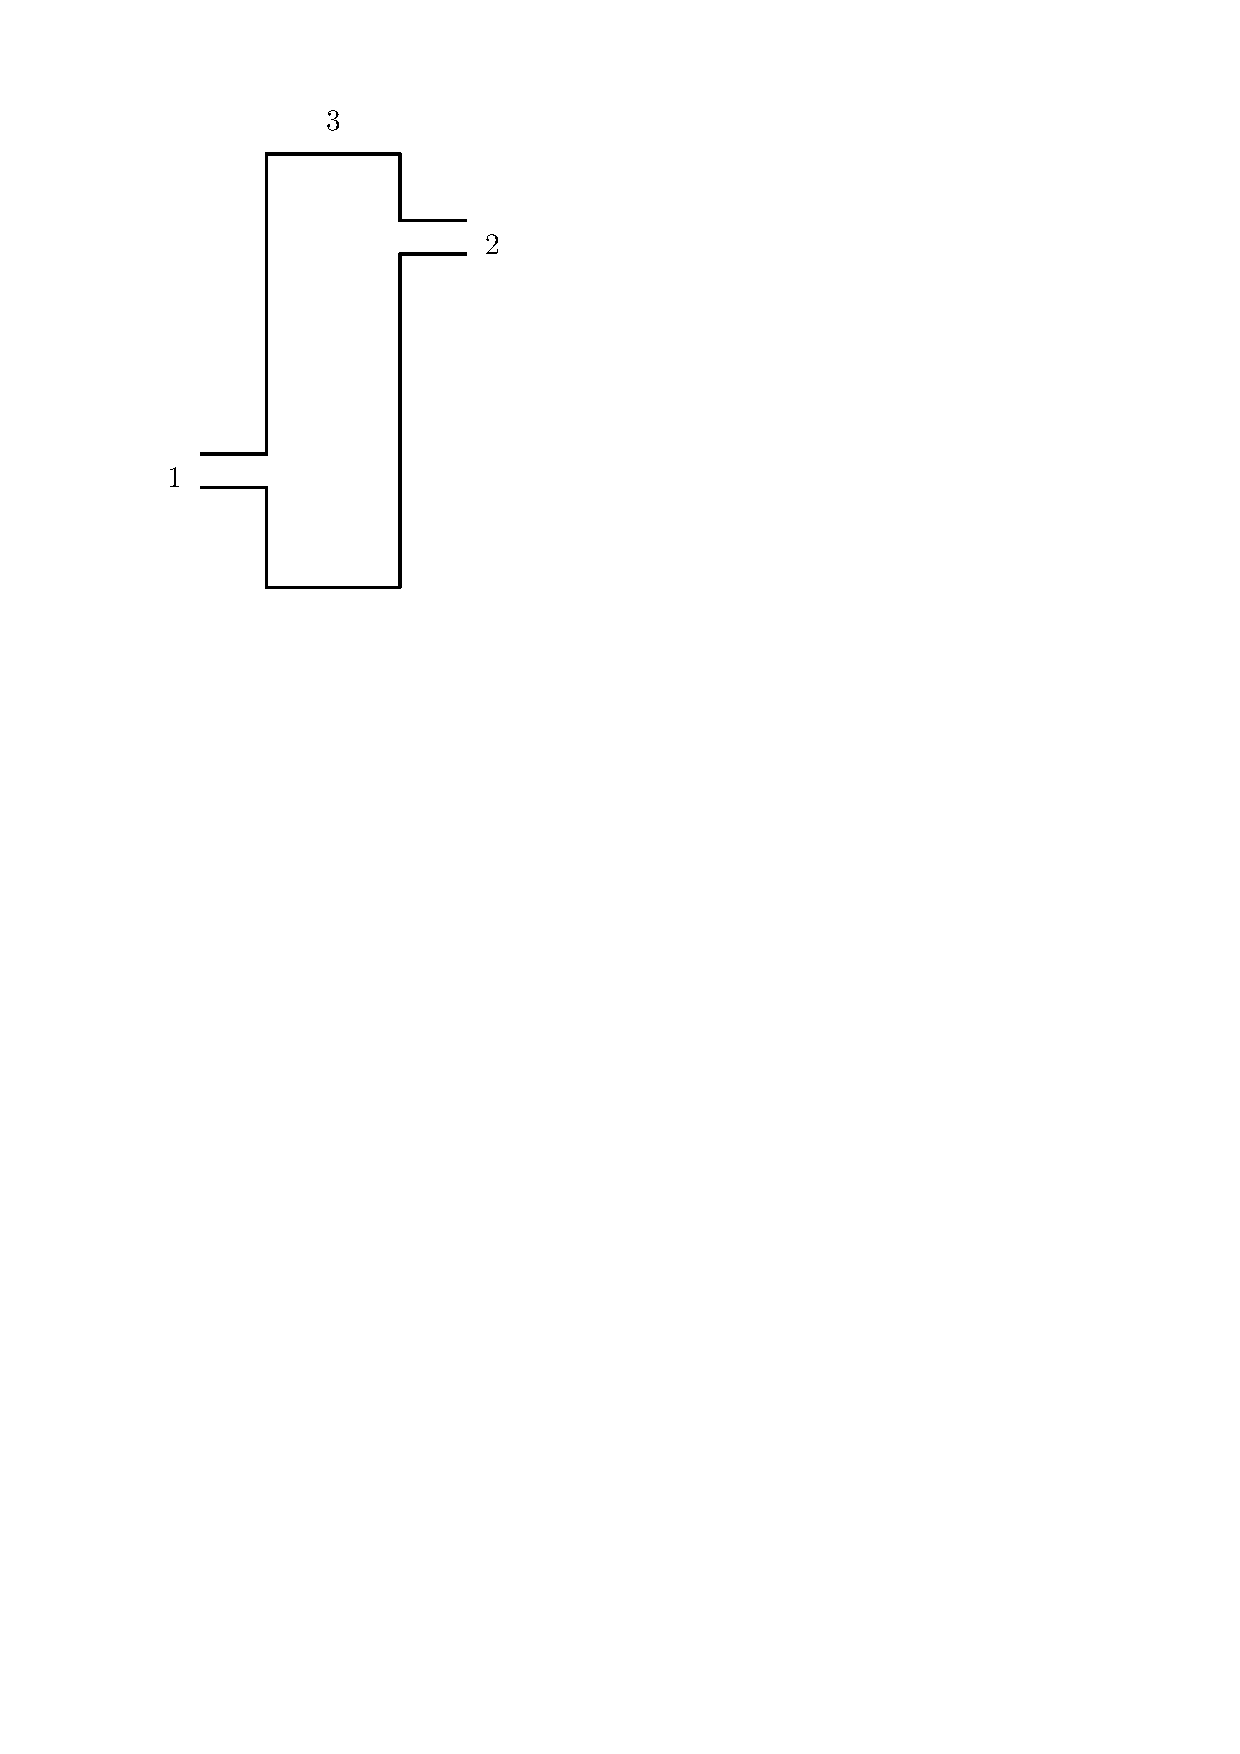
\includegraphics[scale=0.5]{./3.3 Quantità di moto e momento angolare/3.3-1}
		\centering
		\caption{Contenitore con ingressi e uscite concentrati}
	\end{figure}
	%
In caso di approssimazione di ingressi e uscite concentrati, gli integrali vengono divisi nelle parti relative alle tre superfici:
%
	\begin{equation*}
		\oint \uline{r} \cross \uuline{J}_Q \vdot \uline{n} \dd{S} = \int_1 (\ldots) \dd{S} +  \int_2 (\ldots) \dd{S} +  \int_3 (\ldots) \dd{S}
	\end{equation*}
%
Di questi è l'ultimo termine, rappresentante la coppia esercitata sulle pareti, ad essere difficile da calcolare, dato che gli altri due si semplificano supponendo che velocità e pressione siano quasi costanti.

Ad esempio in un  caso stazionario, in cui l'oggetto sia in una posizione tale da annullare il momento esercitato dalla forza di gravità, questo si traduce in:
%
	\begin{equation*}
		\uline{r}_1 \cross (p \uline{n}_1 + \uline{v}_1 \uline{v}_1 \vdot \uline{n}) A_1 + \uline{r}_2 \cross (p \uline{n}_2 + \uline{v}_2 \uline{v}_2 \vdot \uline{n}) A_2 + \textit{coppia sulle pareti} = 0
	\end{equation*}

%SUBSECTION
\subsection{Fattori di correzione per la velocità media}
Una volta fatta l'ipotesi di approssimazione di ingressi e uscite concentrati occorre verificare se questo introduca un errore (e nel caso quantificarlo).
Analizzando in particolare ingressi e uscite si vede che l'ipotesi fatta, della velocità costante e corrispondente al suo valore medio, non è del tutto esatta, dato che la velocità non è costante (tendendo a zero alle pareti per motivi fisici).

Si inizia tramite una rappresentazione del flusso del fluido con un diagramma sovrapposto alle pareti, rappresentante il profilo di velocità.
%
	\begin{figure}[ht]
		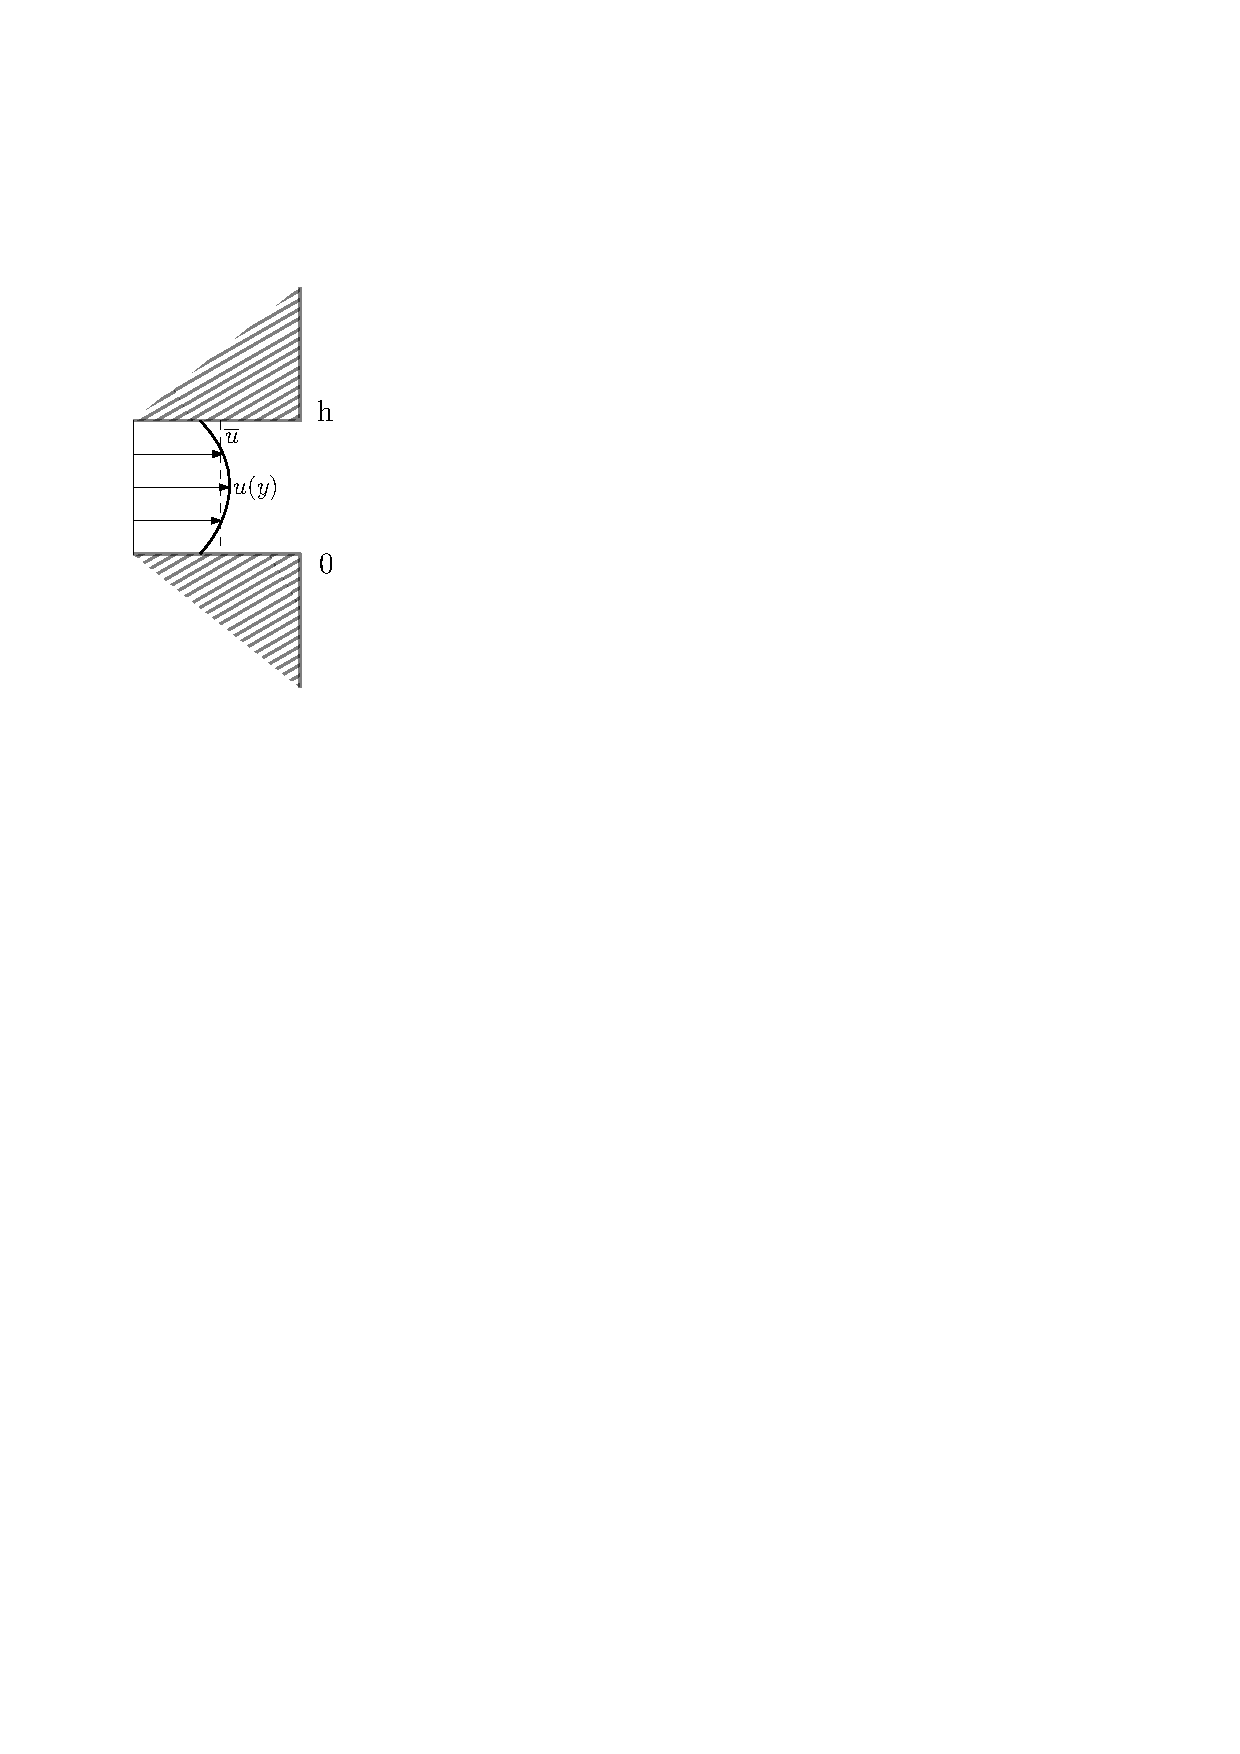
\includegraphics[scale=0.7]{./3.3 Quantità di moto e momento angolare/3.3-2}
		\centering
		\caption{Esempio di profilo di velocità}
	\end{figure}
%
	\begin{figure}[ht]
		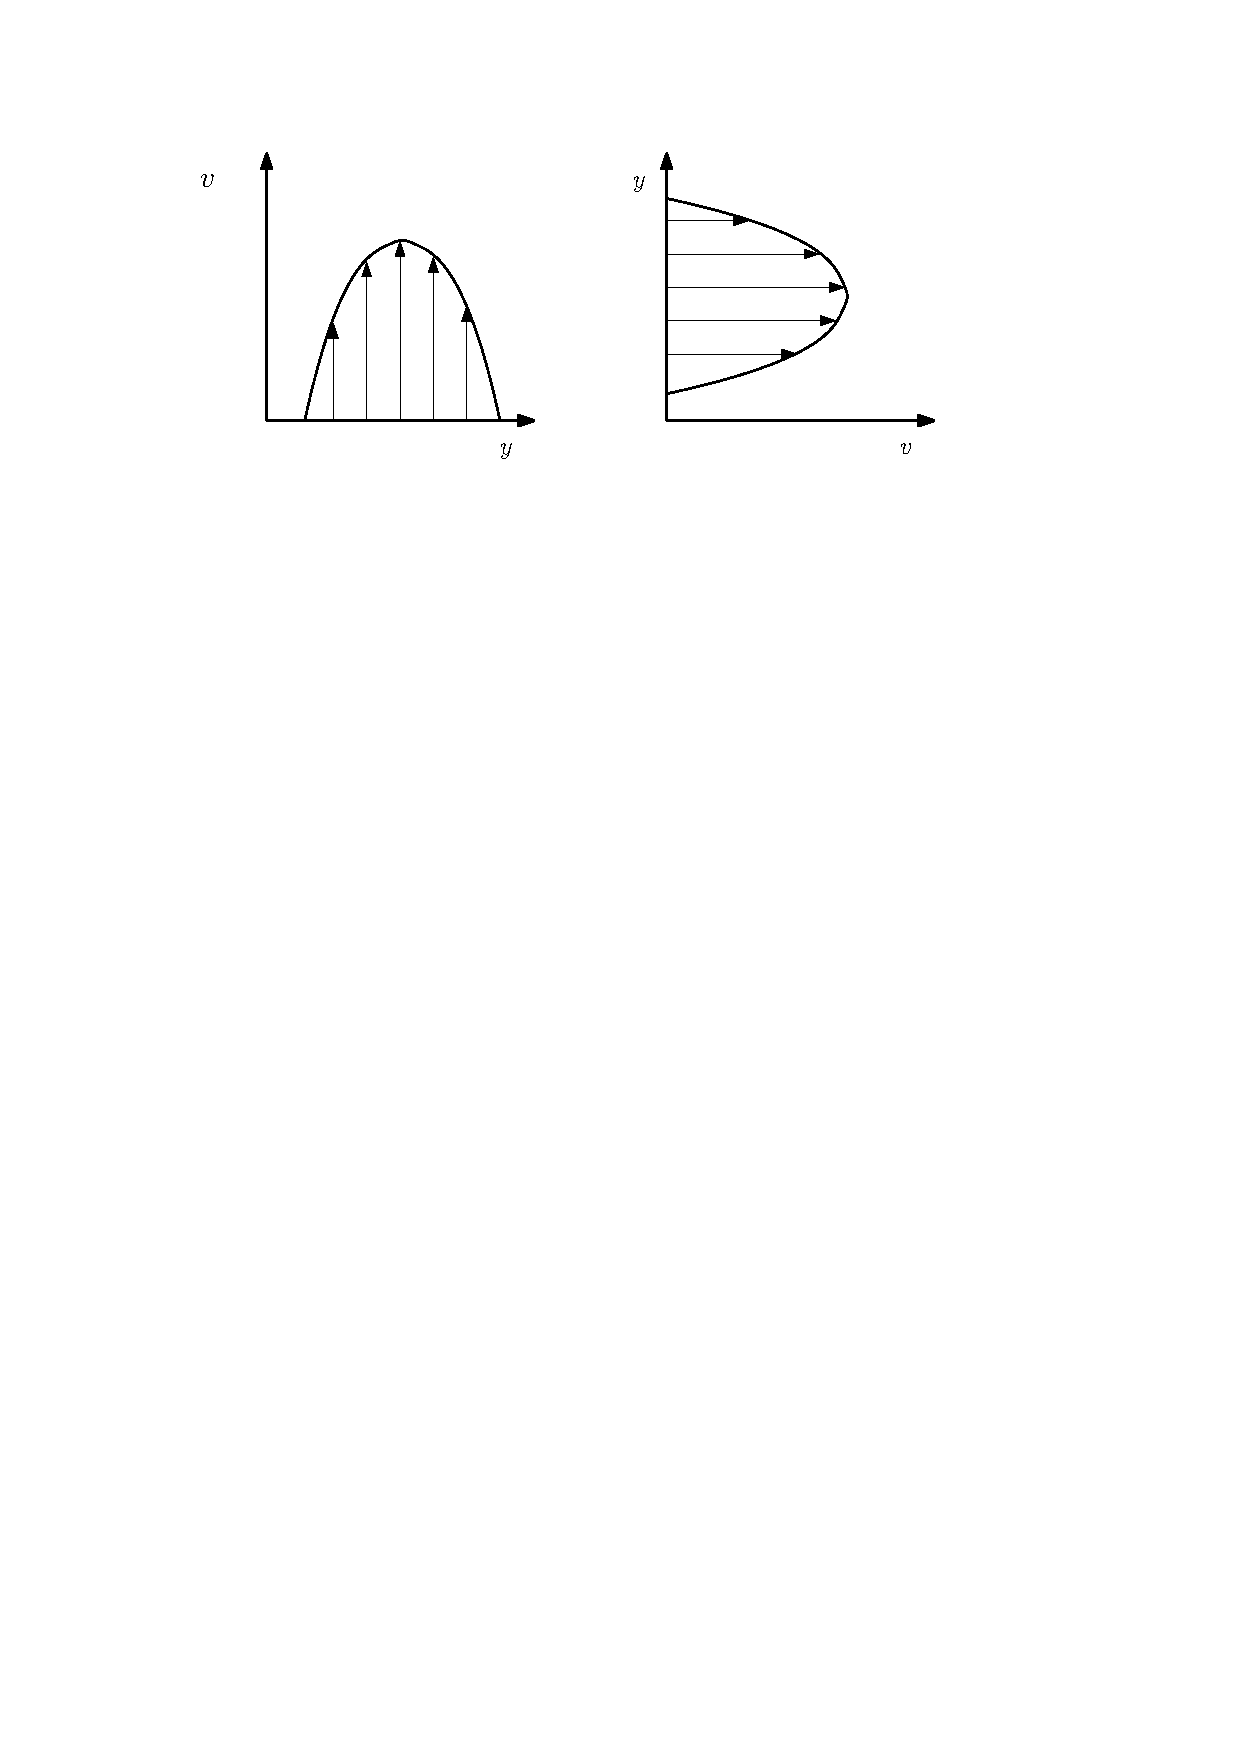
\includegraphics[scale=0.7]{./3.3 Quantità di moto e momento angolare/3.3-3}
		\centering
		\caption{Modulo dei vettori velocità}
	\end{figure}
%
Il profilo di velocità non coincide con il suo valore medio, occorre quindi valutare l'errore commesso con l'approssimazione.
Notare che in questo caso la componente di interesse è una sola, quella della direzione del moto del fluido.

\subsubsection{Massa}
Ad esempio nel flusso di massa occorre calcolare il seguente integrale:
%
	\begin{equation*}
		\int_0^h u(y) \dd{y}
	\end{equation*}
%
Da cui si può definire una costante $\overline{u}$ in modo che valga la seguente:
%
	\begin{equation*}
		\int_0^h u(y) \dd{y} = \overline{u} h
	\end{equation*}
	%
Si vede che questa è la generica definizione di media (quindi l'equazione della massa ``si troverà in automatico'' dato che è usata per definire la costante):
%
	\begin{equation*}
		\overline{u} = \frac{1}{h} \int_o^h u \dd{y} 
	\end{equation*} 
%
	
\subsubsection{Quantità di moto}	
L'integrale seguente appare invece nel calcolo della quantità di moto, ma non è automatico che la definizione di cui sopra valga anche in questo caso:
%
	\begin{equation*}
		\int_0^h (\rho u^2 + P) \dd{y} 
	\end{equation*}
%

Si può suddividere l'integrale in due parti, la prima delle quali sarà ``automaticamente esatta'' una volta definita una pressione media\footnote{tra l'altro una conferma sperimentale di questo ragionamento è data dal fatto che la pressione tende ad essere costante ed avere profili piatti, cosa che non vale per la velocità}:
%
	\begin{equation*}
		\begin{gathered}
			\int_0^h P \dd{y} = \overline{P} h \\
			\int_o^h u^2 \dd{y} \neq \overline{u}^2 h
		\end{gathered}
	\end{equation*}
%
Occorre concentrarsi sul secondo integrale per capire qual è l'errore commesso utilizzando il valore medio della velocità. 
Si introduce quindi un coefficiente adimensionale $\beta$, detto \textbf{fattore di correzione per la quantità di moto}.

Per profili di velocità assegnati a seconda di quanto questo sia diverso da 1 si può valutare l'errore e migliorare il risultato:
%
	\begin{equation*}
		\int_0^h u^2 \dd{y} = \beta \overline{u}^2 h \rightarrow \beta = ?
	\end{equation*}
%
	
\subsubsection{Caso piano laminare}
Uno dei profili più comuni è quello parabolico, ad esempio in un condotto formato da due piani paralleli.
%
	\begin{figure}[ht]
		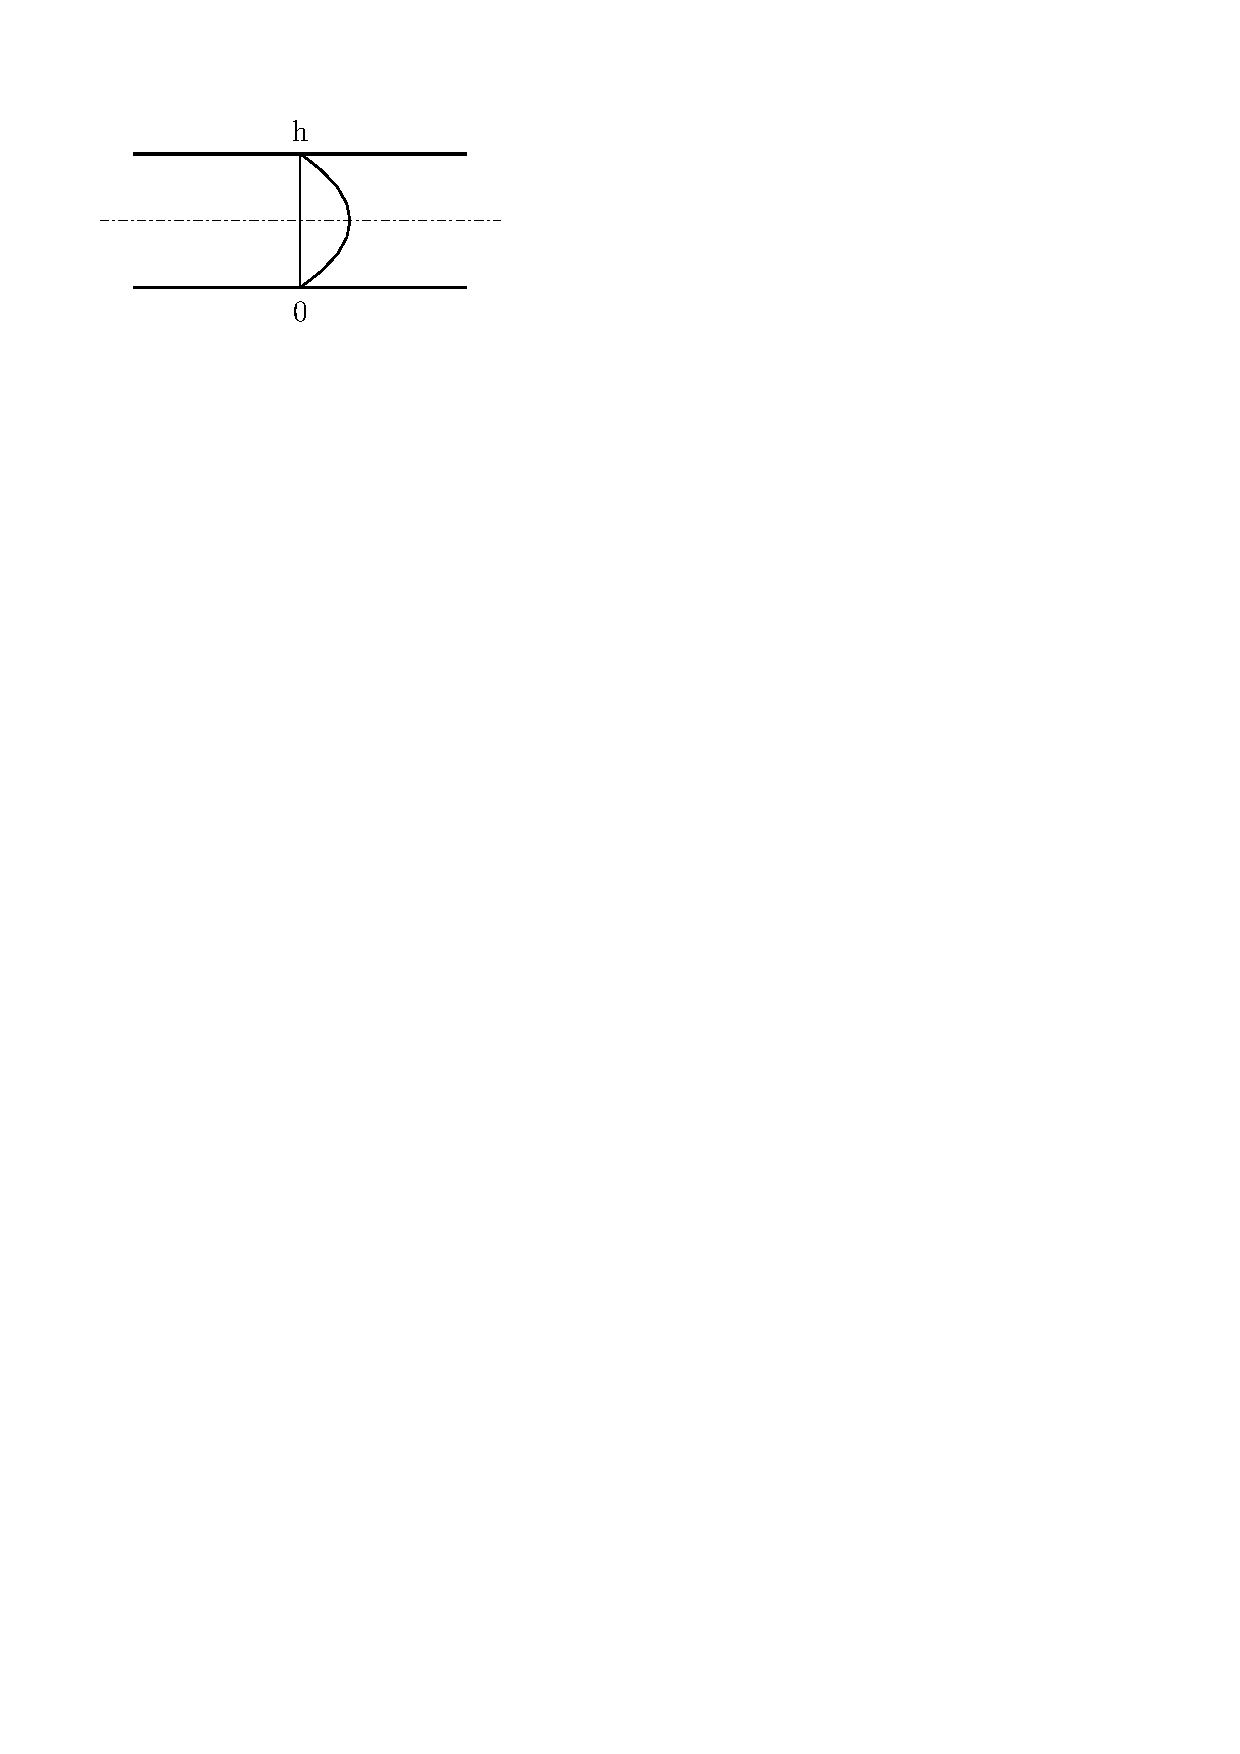
\includegraphics[scale=0.8]{./3.3 Quantità di moto e momento angolare/3.3-4}
		\centering
		\caption{Caso piano laminare}
	\end{figure}
%
Considerando che il profilo è una parabola che va a zero alle pareti, l'unica forma possibile per il profilo di velocità, a meno di un coefficiente A, è:
%
	\begin{equation*}
		u = A y (h - y)
	\end{equation*}
%

È quindi possibile calcolare i due integrali ed il fattore di correzione:
%
	\begin{equation*}
		\begin{gathered}
			\overline{u} = \frac{1}{h} \int_o^h u \dd{y}  = \frac{A}{h} \int_0^h (h y - y^2) \dd{y} = \frac{A h^2}{6} \rightarrow \overline{u}^2 h = \frac{A^2 h^5}{36} \\
			\int_0^h u^2 \dd{y} = A^2 \int_0^h y^2 (h - y) \dd{y} = \frac{A h^5}{30} \\
			\beta =  \frac{\int_0^h u^2 \dd{y}}{\overline{u}^2 h} = \frac{6}{5}
		\end{gathered}
	\end{equation*}
%
Come si può vedere si ha un errore di circa il 20\%, pertanto è meglio tenere conto del fattore di correzione.

\subsubsection{Caso piano turbolento}
Il caso precedente è relativo ad un flusso laminare, cioè in cui le particelle scorrono nella stessa direzione suddivise in lamine.

Nel caso di flusso turbolento, con le particelle che si muovono in direzioni casuali, in maniera disordinata, a parità di geometria cambia il profilo di velocità, che diventa ``più piatto''.
%
	\begin{figure}[ht]
		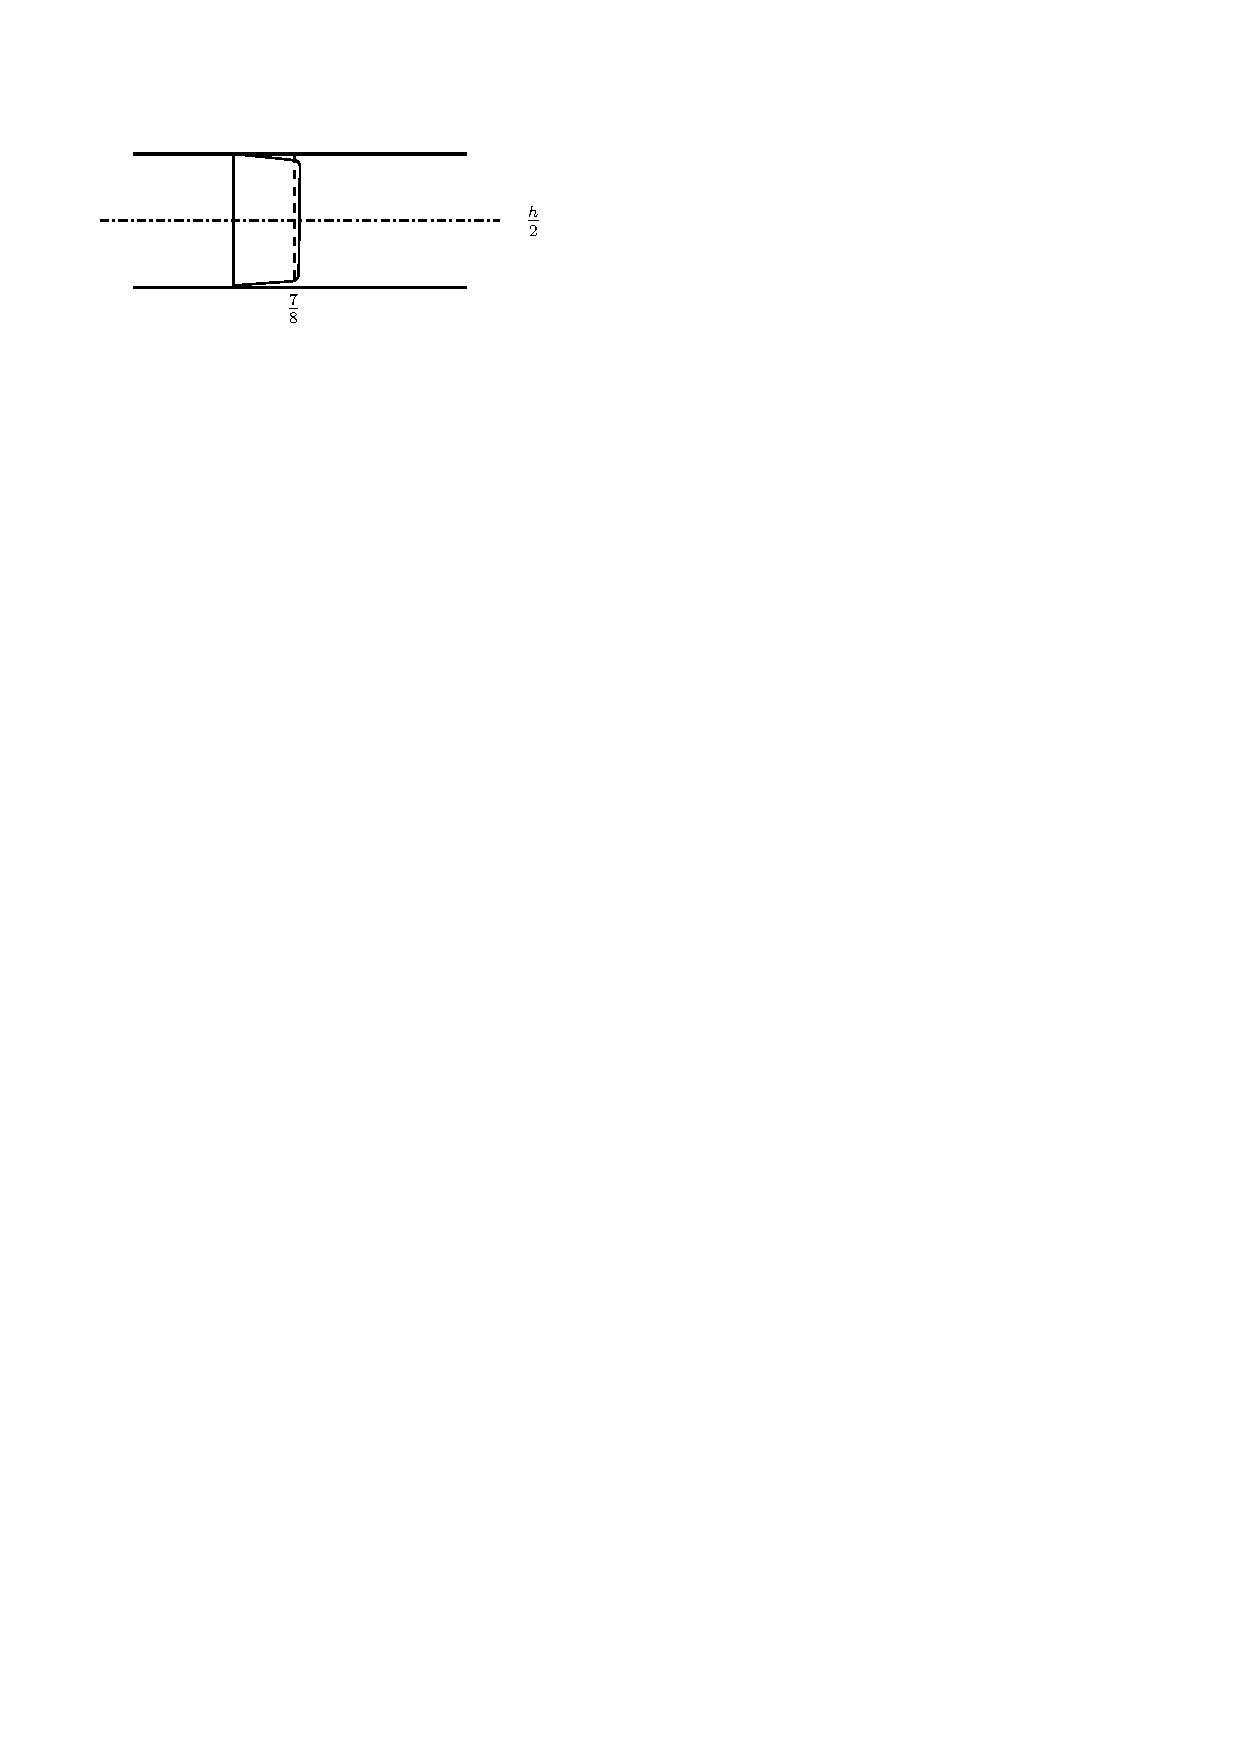
\includegraphics[scale=0.8]{./3.3 Quantità di moto e momento angolare/3.3-5}
		\centering
		\caption{Caso piano turbolento}
	\end{figure}
%

Una delle prime approssimazioni empiriche per definire questo profilo è:
%
	\begin{equation*}
		u = A y^{\frac{1}{7}} \quad \textit{per} \quad 0 < y < \frac{h}{2} \quad \textit{(ribaltata per l'altra metà profilo)}
	\end{equation*}
%
Da questo segue:
%
	\begin{equation*}
		\begin{gathered}
			\overline{u} = \frac{1}{h} \int_o^h u \dd{y} = \frac{2}{h} \int_0^{\frac{h}{2}} a y^{\frac{1}{7}} \dd{y} \rightarrow \overline{u}^2 \frac{h}{2} = A^2 {\qty(\frac{h}{2})}^{\frac{9}{7}} \frac{49}{64} \\
			\int_0^{\frac{h}{2}} u^2 \dd{y} = A^2 \int_0^{\frac{h}{2}} y^{\frac{2}{7}} \dd{y} = \frac{7}{9} A^2 {\qty( \frac{h}{2})}^{\frac{9}{7}}
		\end{gathered}
	\end{equation*}
%			
Infine:			
%
	\begin{equation*}
			\beta = \frac{\int_0^{\frac{h}{2}} u^2 \dd{y}}{\overline{u}^2 \frac{h}{2}} = \frac{64}{63}
	\end{equation*}
%
Considerando che si è già in una situazione approssimata, dato che $\beta$ si avvicina ad 1 può essere trascurato.

\subsubsection{Caso cilindrico laminare}
Altro caso di interesse è quello in cui si abbia una geometria cilindrica (ad esempio un tubo).
%
	\begin{figure}[ht]
		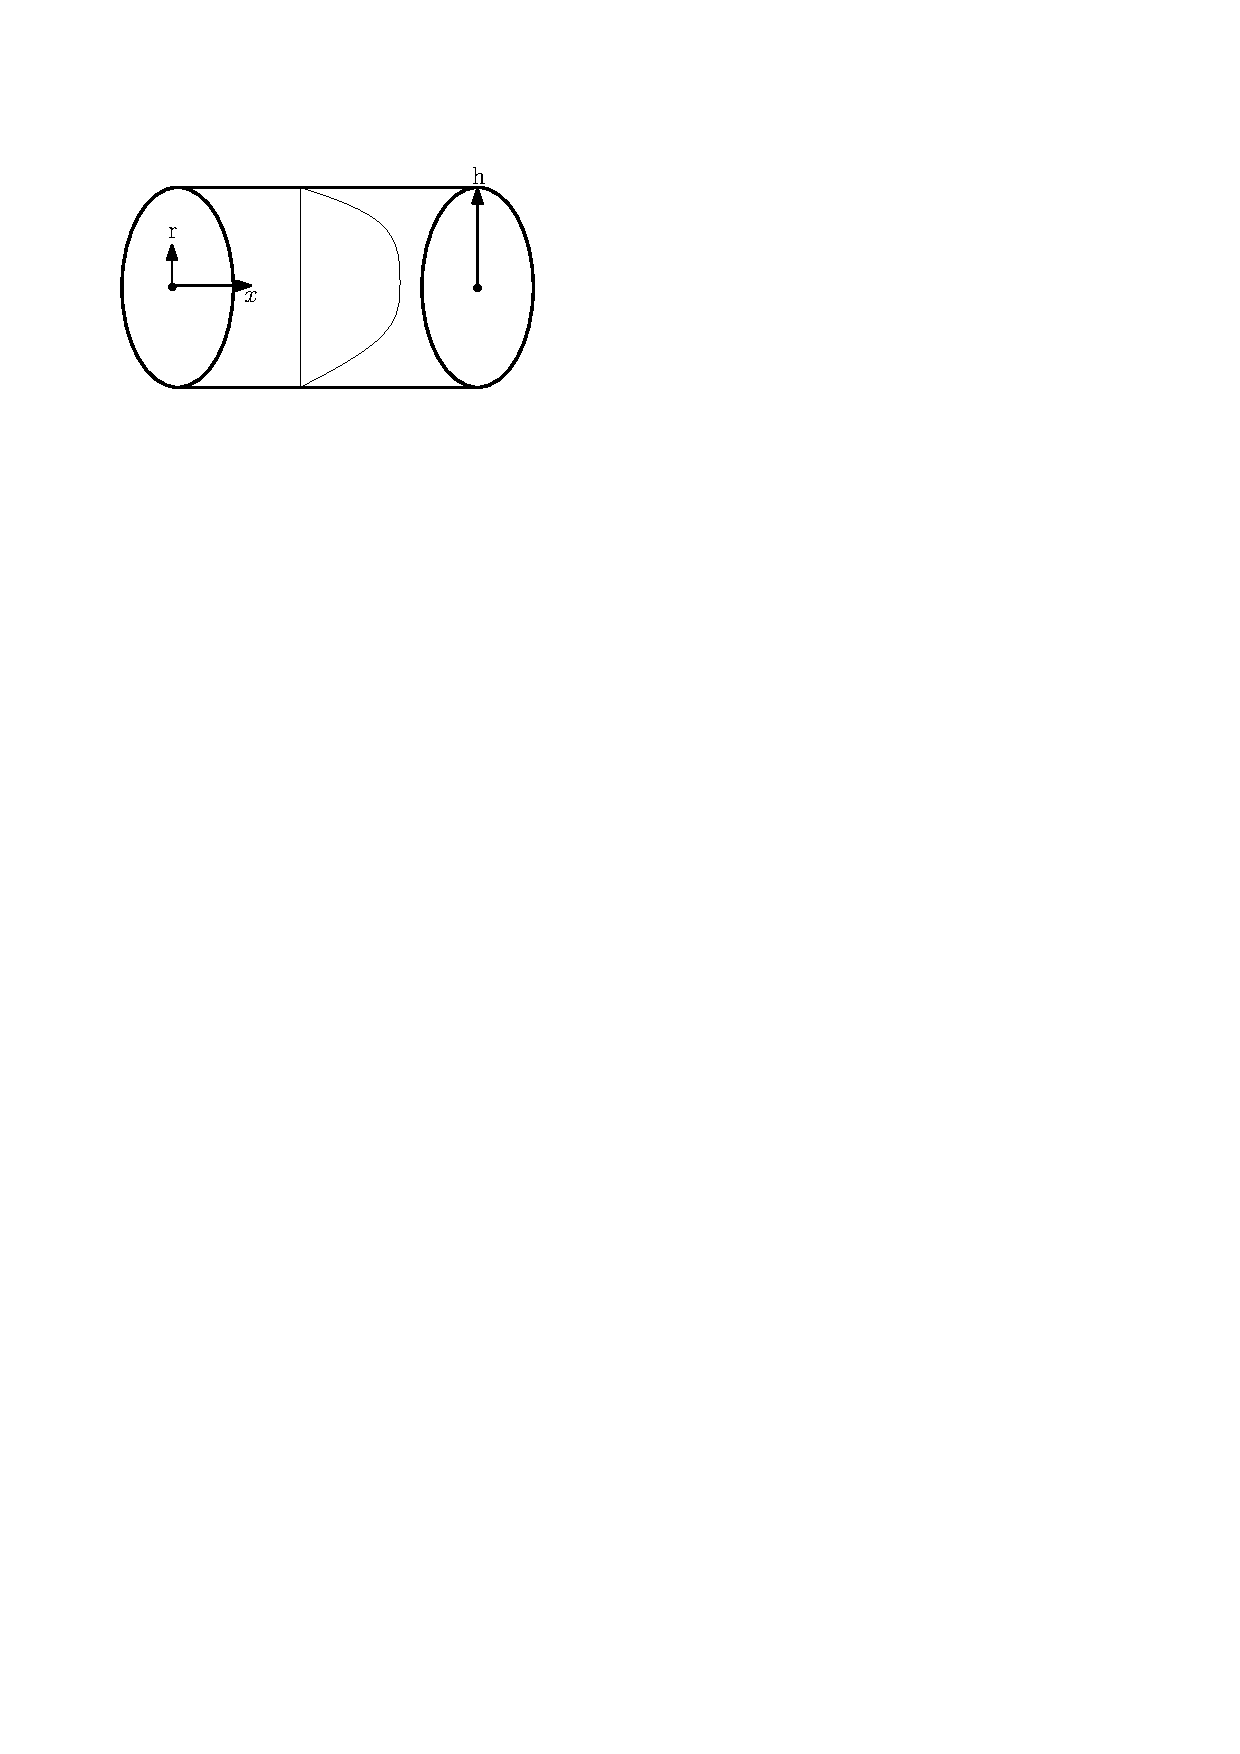
\includegraphics[scale=0.80]{./3.3 Quantità di moto e momento angolare/3.3-6}
		\centering
		\caption{Caso cilindrico laminare}
	\end{figure}
%

Il procedimento è analogo a quello piano (il profilo di velocità è nuovamente parabolico), tenendo conto che in questo caso si integra su una superficie cilindrica ($2 \pi r \dd{r}$) e per la media bisogna dividere per l'area ($\pi h^2$):
%
	\begin{equation*}
		\begin{gathered}
			u(r) = A  \qty(1 - \frac{r^2}{h^2}) \\
			\overline{u} = \frac{1}{\pi h^2} \int_0^h A  \qty(1 - \frac{r^2}{h^2}) 2 \pi r \dd{r} = \frac{A}{2} \rightarrow \overline{u}^2 \pi h^2 = \frac{\pi A^2 h^2}{4} \\
			\int_0^h u^2 2 \pi r \dd{r} = 2 \pi A^2 \int_0^h \qty(1 -2 \frac{r^2}{h^2} + \frac{r^4}{h^4}) r \dd{r} = \frac{\pi A^2 h^2}{3} \\
			\beta = \frac{\int_0^h u^2 2 \pi r \dd{r}}{ \overline{u}^2 \pi h} =\frac{4}{3}
		\end{gathered}
	\end{equation*}
%
In questo caso $\beta$ non è trascurabile, l'errore commesso sarebbe di circa il 33\%.

\subsubsection{Caso cilindrico turbolento}
%
	\begin{figure}[ht]
		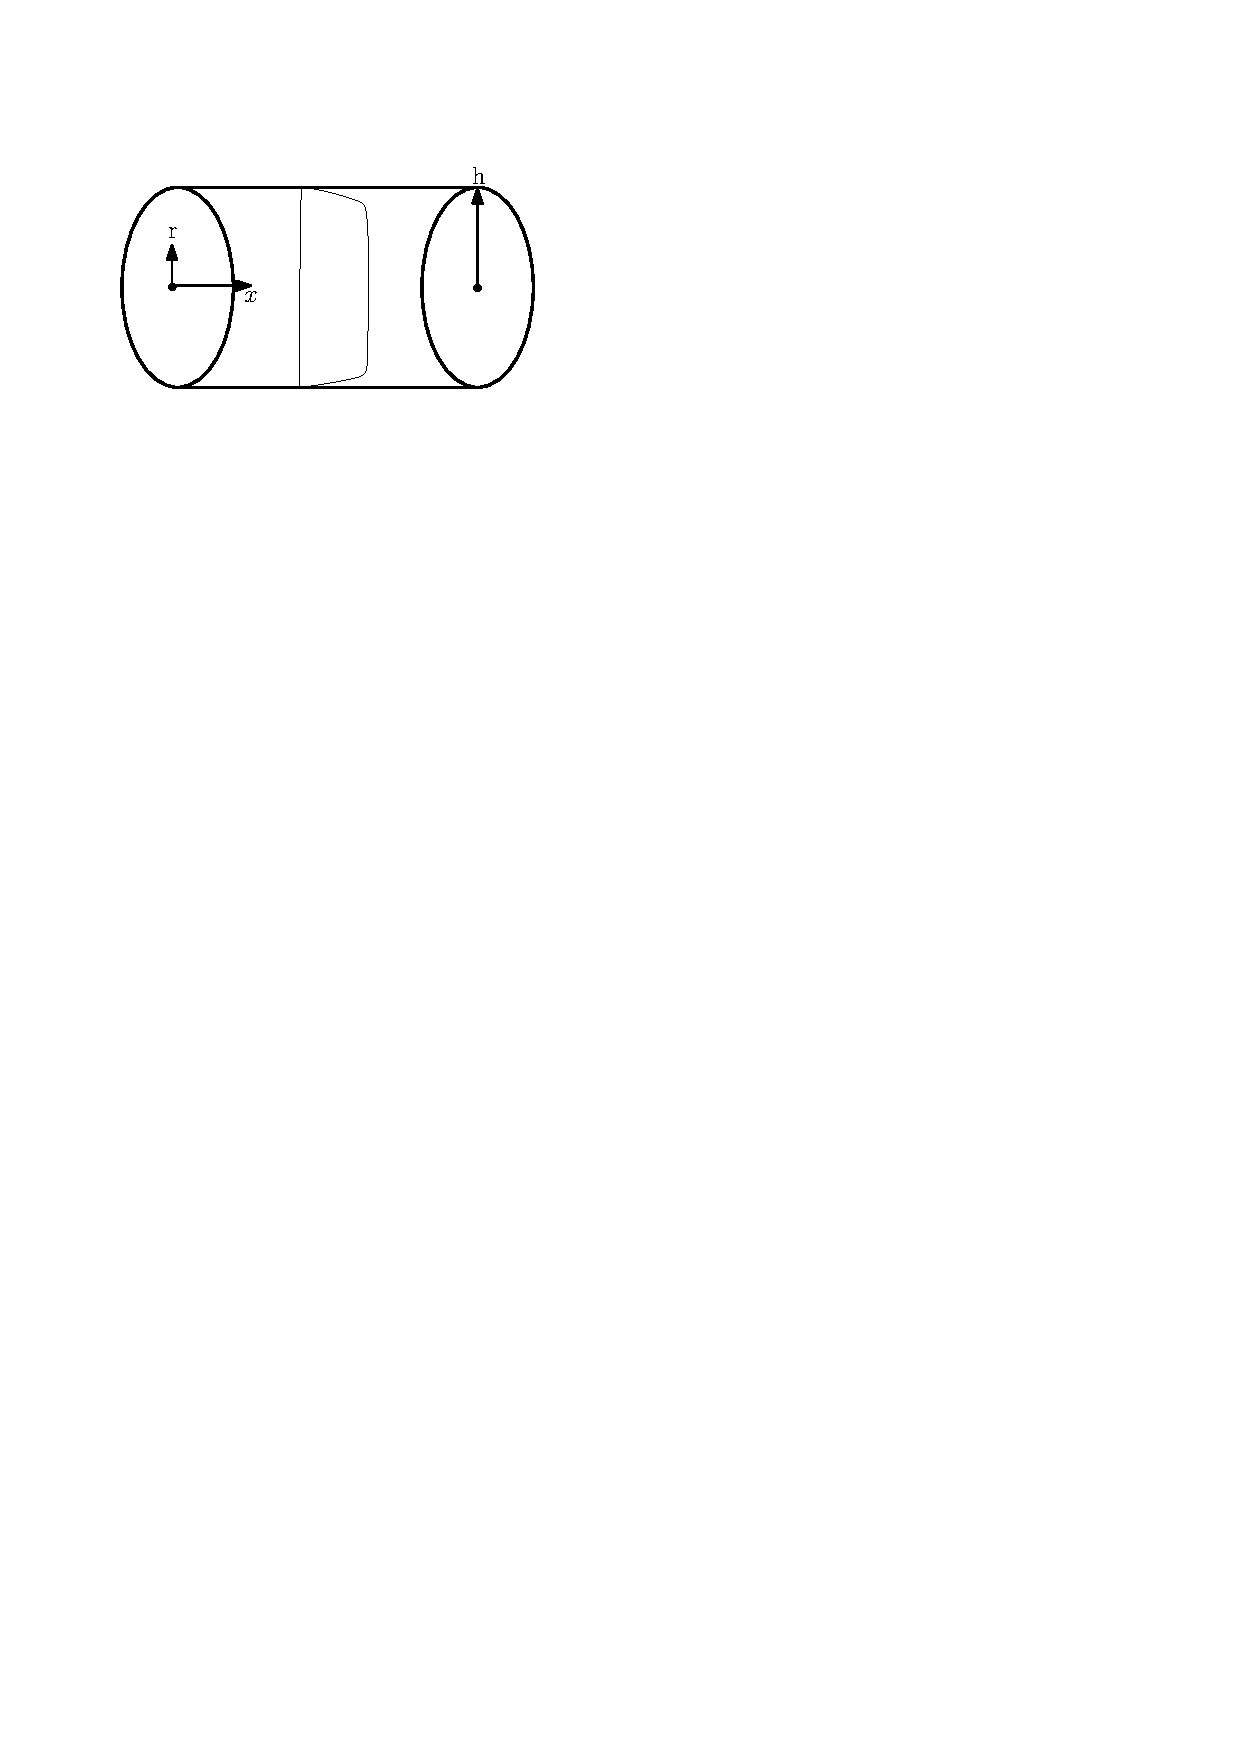
\includegraphics[scale=0.80]{./3.3 Quantità di moto e momento angolare/3.3-7}
		\centering
		\caption{Caso cilindrico turbolento}
	\end{figure}
%

Si procede analogamente al caso piano, tenendo conto della geometria differente.
 Definito $y = h - r$ (dato che il profilo di velocità è definito è a partire dal bordo) si ha che:
%
	\begin{equation*}
		\begin{gathered}
			u = A y^{\frac{1}{7}} \\
			\overline{u} = \frac{1}{\pi h^2} \int_0^h A y^{\frac{1}{7}} 2 \pi r \dd{r} = \frac{1}{\pi h^2} \int_0^h A y^{\frac{1}{7}} 2 \pi (h - y) \dd{r} = \frac{49}{60} A h^{\frac{1}{7}} \rightarrow \\
			\rightarrow \pi h^2 \overline{u}^2 = \pi a^2 h^\frac{16}{7} {\qty( \frac{49}{60})}^2 \\
			\int_0^h u^2 2 \pi r \dd{r} = 2 \pi \int_0^h A^2 y^{\frac{2}{7}} (h - y) \dd{y} = \pi A^2 h^{\frac{16}{7}} \frac{49}{72} \\
			\beta = \frac{\int_0^h u^2 2 \pi r \dd{r}}{\pi h^2 \overline{u}^2} = \frac{50}{49}
		\end{gathered}
	\end{equation*}
%
Anche in questo caso $\beta$ è trascurabile.

\subsection{Tabella riassuntiva coefficienti di correzione per la quantità di moto}
%
	\begin{table}[H]
		\begin{tabular}{ccc}
			\toprule
				\textit{Geometria}/\textbf{Moto}	&	\textbf{Laminare}	&	\textbf{Turbolento}\\
			\midrule
				\textit{Piana}		&	$\frac{6}{5}$	&	$\frac{64}{63}$ \\
			\midrule
				\textit{Cilindrica} 	&	$\frac{4}{3}$	&	$\frac{50}{49}$\\
			\bottomrule
		\end{tabular}
	\end{table}
%
Notare che il coefficiente di correzione è sempre maggiore o uguale ad uno, dato che l'integrale è sempre maggiore della media.
Inoltre notare come nei casi turbolenti sia trascurabile, mentre nei casi laminari conviene inserirlo dato che è un numero ``fisso'' e non complica di molto i calcoli.

\subsection*{Bibliografia 3.4}
\cite[Cap.\ 4.5, 4.6, 4.7, 4.85.1, 5.2]{CengelCimbala}\\
\cite[Cap.\ 6.4]{PnueliGutfinger}